%%%%%%%%%%%%%%%%%%%%%%%%%%%%%%%%%%%%%%%%%%%%%%%%%%%%%%%%%%%%%%%%%%%%%%%%%%%%%%%%%%%%%%%%%
% Appendix B: FamilyInfo XML Files
%	This section provides a detailed description of Family Info files, and their
%   syntax. Most users of RapidSmith2 don't need to know the syntax of family info
%   files, but this information may be useful to new lab members working on the
%   project.
%%%%%%%%%%%%%%%%%%%%%%%%%%%%%%%%%%%%%%%%%%%%%%%%%%%%%%%%%%%%%%%%%%%%%%%%%%%%%%%%%%%%%%%%%
\newpage
\section{Family Info XML} \label{sec:familyInfo}

A \textit{familyInfo.xml} file contains useful information that is
not present in the XDLRC files for a given family of devices. Specifically, it
includes the following additional information about each site type in a family:

\begin{multicols}{2} 
	\begin {itemize}
      \item \textbf{Alternate Types}
      \item \textbf{Compatible Types}
      \item \textbf{BEL Routethroughs}
      \item \textbf{Site PIP Corrections}
      \item \textbf{Pin Direction Corrections}
	\end{itemize}
\end{multicols}

\noindent 
As the name suggests,  only one \textit{familyInfo.xml} is required for each of
the supported Vivado families listed in \autoref{tab:vivadoFamilies} (all
devices within a family share the same family info).  A new \texttt{Tincr}
command has been added to generate family info files:
\texttt{[tincr::create\_xml\_family\_info]}.  Using this command, with a few
required hand edits, \textbf{a complete set of family info XML files have been
created for all Series7 and UltraScale families}.  The following subsections
describe each component of a family info XML and why they may be useful for
external CAD tools.

\subsection{Alternate Types} \label{sec:alternateSites}
Each physical site in a device has an associated default type. Some sites,
however, can be configured to be one of many types (called alternate
types in Vivado). Alternate type information is required for external CAD tools because
the type of a site can be changed during the placement phase of implementation.
To accurately represent a placed design in an external tool, site types need to
be changeable. An example of alternate types for an UltraScale BITSLICE\_RX\_TX
site is shown in \autoref{fig:alternateTypes}. As the figure shows, a
BITSLICE\_RX\_TX site can also be configured to be of type
BITSLICE\_COMPONENT\_RX\_TX, BITSLICE\_RXTX\_RX, or BITSLICE\_RXTX\_TX.
\autoref{lst:familyInfoAlternate} shows how alternate types are
represented in a family info XML. Pinmap tags are included for alternate pin
names changing as decribed in \autoref{sec:series7HandEdits}.

\begin{figure}[b!]
  \centering
  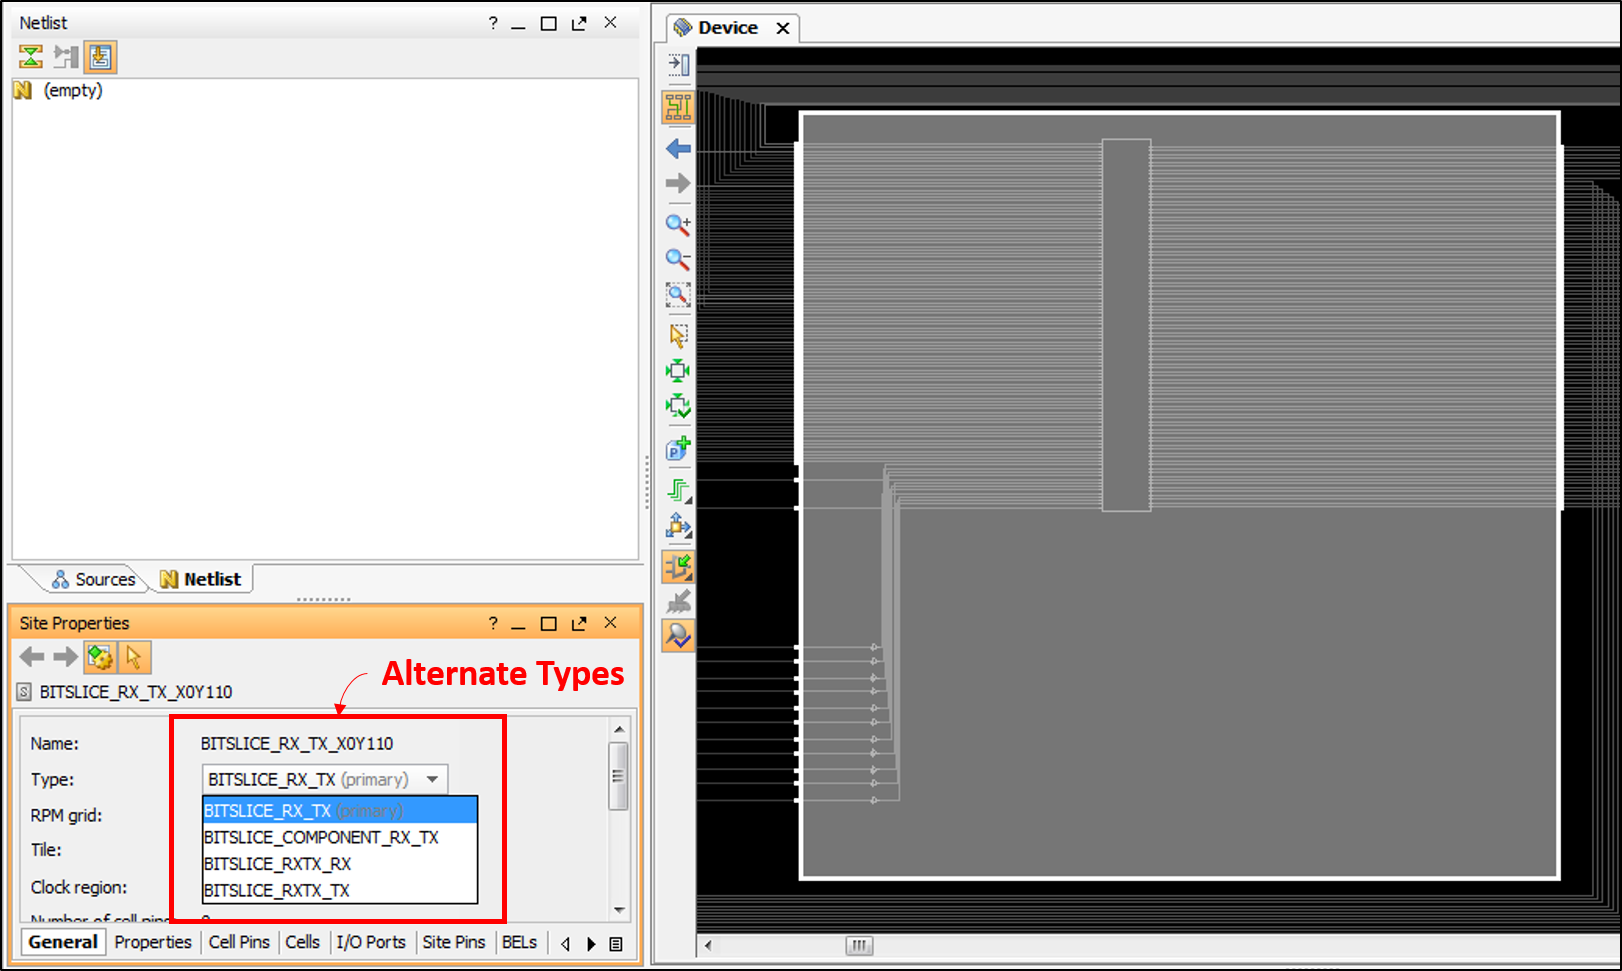
\includegraphics[width=.6\columnwidth]{alternateTypes.png}
  \caption{BITSLICE\_RX\_TX Alternate Types}
  \label{fig:alternateTypes}
\end{figure}

\begin{lstlisting}[numbers=none, keywordstyle=, stringstyle=, caption=Example
Alternate Type XML, label=lst:familyInfoAlternate] 
  <alternative>
      <name>ISERDESE2</name>
      <pinmaps>
          <pin>
	          <name>RST</name>
              <map>SR</map>
	      </pin>
      </pinmaps>
  </alternative>
\end{lstlisting}

\subsection{Compatible Types}
Site \texttt{A} is said to be compatible with site \texttt{B} if the logical
cells placed on site \texttt{A} can \textit{always} be placed on site \texttt{B}
as well. For example, as shown in \autoref{fig:sliceCompatibility}, SLICEL sites
are compatible with SLICEM sites. The cells placed on the SLICEL in the figure
can be moved to the SLICEM and still function identically. SLICEMs, however,
are \textit{not} compatible with SLICELs. This is because SLICEM sites support
LUT RAM cells, which cannot be placed on SLICEL sites.  In some cases of
compatibility, the type of the compatible site must first be changed before
placing cells on it. For instance, a RAMB36 site is compatible with a
RAMBFIFO36 site, but the site type of the RAMBFIFO36 \textbf{must
first be changed to RAMB36} before it is truly compatible. 

\begin{figure}[h!]
  \centering
  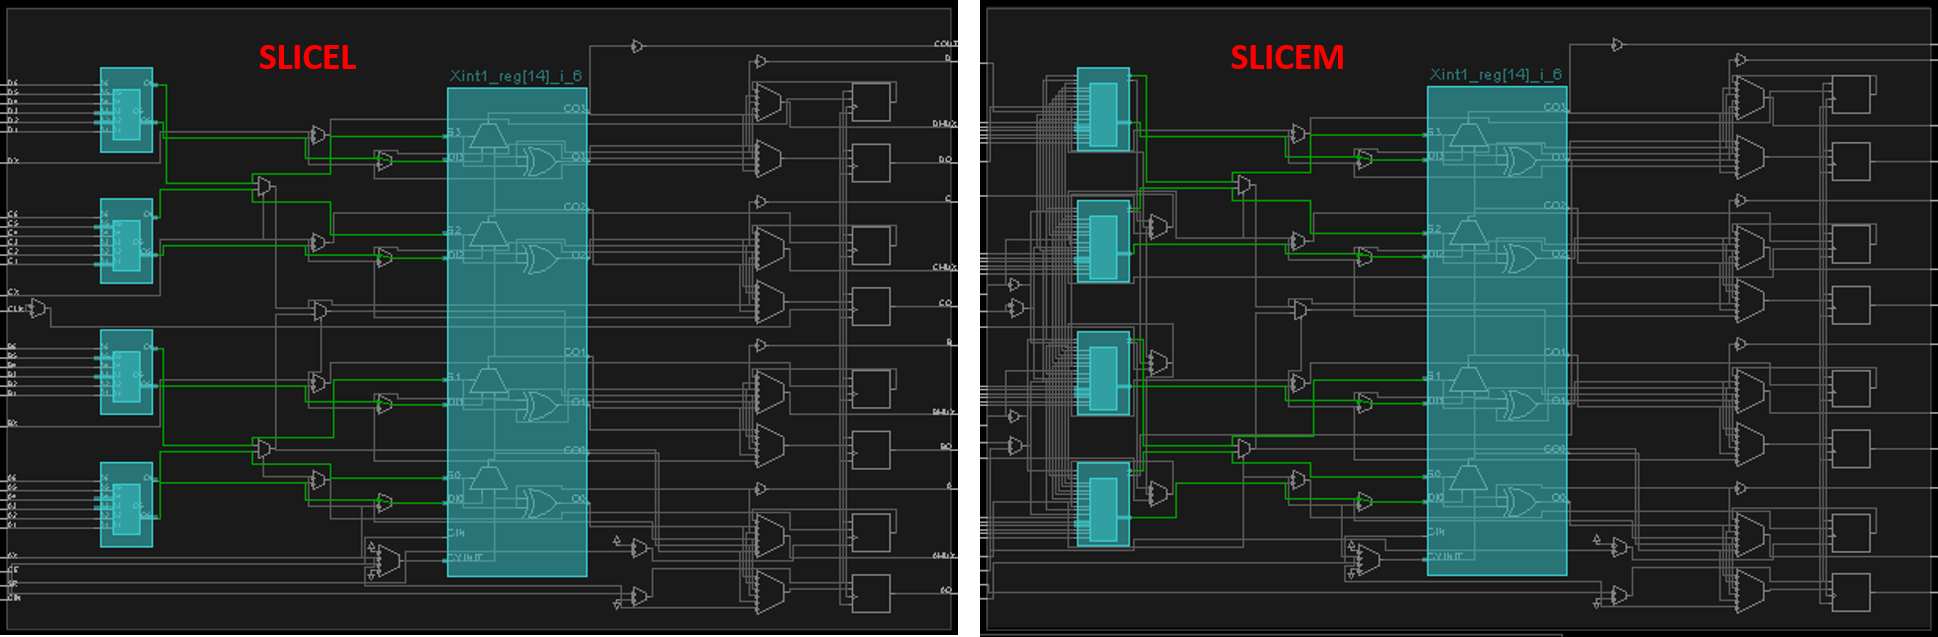
\includegraphics[width=1\columnwidth]{compatibleSites.png}
  \caption{A group of cells placed on a SLICEL site (left) and a SLICEM
  site (right).}
  \label{fig:sliceCompatibility}
\end{figure}

\begin{figure}[b!]
  \centering
  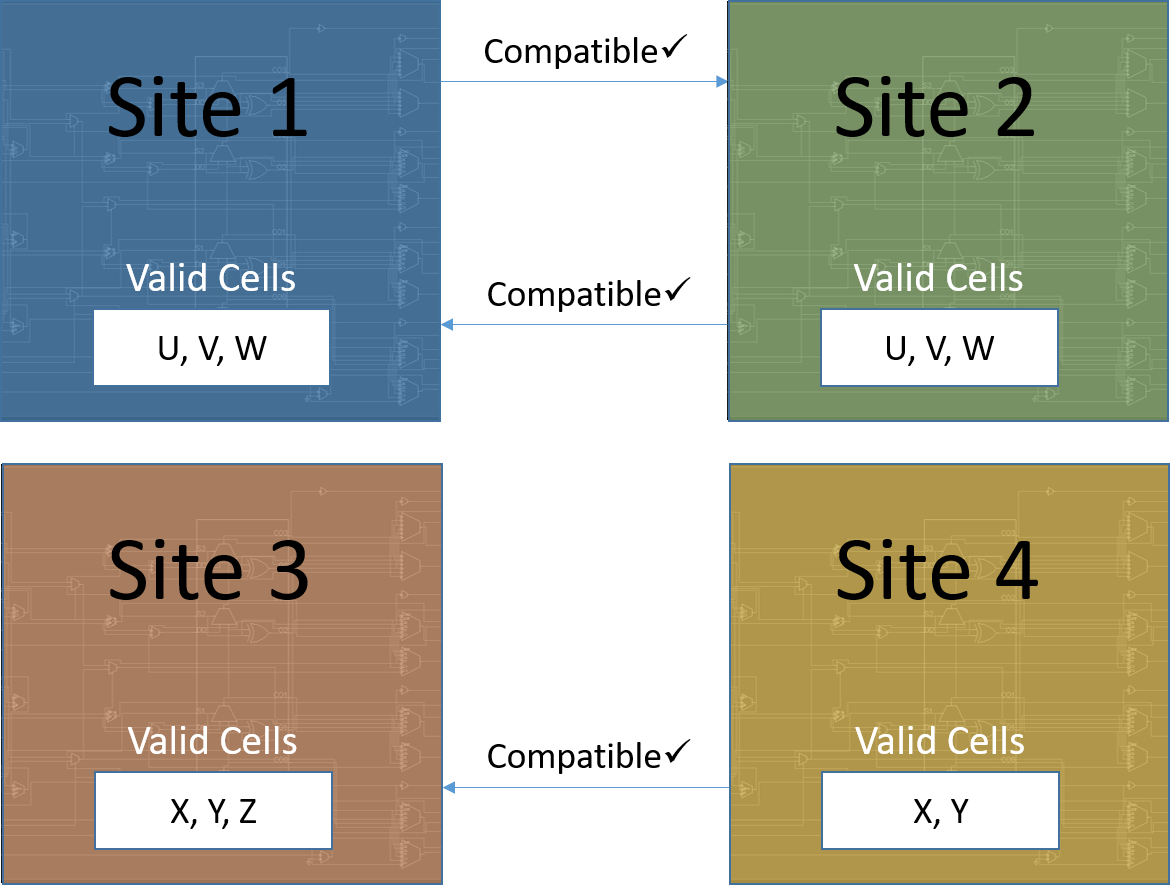
\includegraphics[width=.6\columnwidth]{compatibleTest.png}
  \caption{Compatibility Testing for Single-BEL Sites}
  \label{fig:singleBelCompatibleTest}
\end{figure}

A visualization of compatibility is also given in
\autoref{fig:singleBelCompatibleTest}. In this case, ``Site 1'' and ``Site 2''
are both compatible to each other since the same set of cells can be placed
onto both sites. ``Site 4'' is compatible with ``Site 3'' because each cell that
can be placed on ``Site 4'' can also be placed on ``Site 3.'' ``Site 3'', however, is
not compatible with ``Site 4'' because cell \texttt{Z} cannot be placed on
``Site 4.''

Information about compatible types is useful in a variety of CAD applications.
One such application is a site-level placer. To achieve the best
placement results, the placer needs to understand \emph{all} available
locations where a set of cells can be placed. Without information about
compatible types, the placer would only know how to target one specific site
type for each group of cells, lowering the quality of results.
\autoref{lst:compatibleTypes} shows example XML for compatible types in a
family info file.

\begin{lstlisting}[numbers=none, keywordstyle=, stringstyle=,
caption=Compatible Type XML for SLICEL, label=lst:compatibleTypes]
  <compatible_types>
    <compatible_type>SLICEM</compatible_type>
  </compatible_types>
\end{lstlisting}

\subsection{BEL Routethroughs}
During the routing stage of implementation, certain BELs can be configured as
PIPs in a device (i.e. they pass a signal from an input pin directly to an
output pin). To fully represent the routing structure within
a Xilinx FPGA, these \textbf{routethrough} connections are included in the
family info file. \autoref{lst:familyInfoRoutethrough} shows how routethrough
connections are represented. External tools can use this information to
build a more accurate device data structure. At the time of writing, BELs are
considered routethrough candidates if they are of type ``LUT" or ``Flip-Flop"
on a SLICE site. A more detailed discussion of routethroughs is presented in
\autoref{sec:belRoutethroughs}.

\begin{lstlisting}[numbers=none, keywordstyle=, stringstyle=,
caption=Example Routethrough XML, label=lst:familyInfoRoutethrough]
  <bel>
      <name>D6LUT</name>
      <type>LUT6</type>
      <routethroughs>
          <routethrough>
              <input>A1</input>
              <output>O6</output>
          </routethrough>
          <routethrough>
              <input>A2</input>
              <output>O6</output>
          </routethrough>
      <routethroughs>
  </bel>
\end{lstlisting}

\subsection{Site PIP Corrections}
XDLRC files do not distinguish the difference between site PIPs (routing muxes)
and functional BELs within a site. Each of these components are simply marked
as a ``Bel'', even though site PIPs are certainly not BELs. The family info file
corrects this by explicitly marking site PIPs as \textbf{routing muxes} or
\textbf{polarity selectors}. A polarity selector is a site PIP with one
input that can be optionally inverted. \autoref{lst:pipCorrectionXml} shows how
site PIP corrections are represented in a family info file.

\begin{lstlisting}[numbers=none, keywordstyle=, stringstyle=,
caption=Example Site PIP Corrections, label=lst:pipCorrectionXml]
  <corrections>
      <modify_element> 
          <name>A5FFMUX</name> 
          <type>mux</type> 
      </modify_element>
      <polarity_selector> 
          <name>CLKINV</name> 
      </polarity_selector>
  </corrections>
\end{lstlisting}

\noindent RapidSmith2 decomposes a site PIP into its individual PIPs as shown in
\autoref{fig:sitePipDecomposition}. This decomposition generally makes creating
routing algorithms easier. In Vivado, site PIPs are determined with the Tcl
command \texttt{[get\_site\_pips -of \$site]}. Polarity selectors are
distinguished from regular site PIPs by checking if the string name of the PIP
ends with either ``INV'' or ``OPTINV''.
  
\begin{figure}[H]
  \centering
  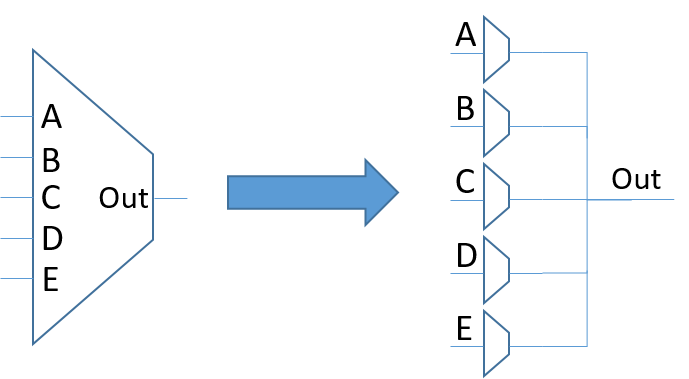
\includegraphics[width=.6\columnwidth]{sitePipDecomposition.png}
  \caption{Site PIP Decomposition}
  \label{fig:sitePipDecomposition}
\end{figure}

\subsection{Pin Direction Corrections}
In XDLRC files, all BEL pins are given a direction of either INPUT or OUTPUT.
However, there are several BEL pins in Xilinx devices that are of direction
INOUT (bidirectional). The family info file marks INOUT BEL pins so that their
direction can be corrected in RapidSmith2. The direction of a BEL pin in
Vivado can be determined with the Tcl command \texttt{[get\_property DIRECTION
\$belpin]}. \autoref{lst:pindirCorrectionXml} shows how pin direction
corrections are represented in XML.

\begin{lstlisting}[numbers=none, keywordstyle=, stringstyle=,
caption=Example Pin Direction Correction, label=lst:pindirCorrectionXml]
  <corrections>
      <pin_direction>
          <element>PAD</element>
          <pin>PAD</pin>
          <direction>inout</direction>
      </pin_direction>
  </corrections>
\end{lstlisting}